\documentclass[12pt, a4paper]{ctexart}
\usepackage{CJK}
\usepackage{graphicx, natbib}
\DeclareGraphicsExtensions{.eps,.ps,.jpg,.bmp}
\usepackage{indentfirst, amsmath}
\usepackage{tikz}
\usepackage{fancyhdr}
\usepackage{epstopdf}
\pagestyle{fancy}
\lhead{}
\rhead{}
\chead{\fangsong 材料力学课程研究报告} 
\cfoot{}
\rfoot{\thepage} 
\renewcommand{\headrulewidth}{0.4pt} 
\renewcommand{\footrulewidth}{0pt}


\newcommand{\thistitle}{拉压断面分析}
\newcommand{\thisauthor}{吴思源}


\title{\thistitle}
\author{\thisauthor}
\begin{document}
%%%%%%%%%%%%%%%%%%%%%%%%%%%%%%
%% 封面部分
%%%%%%%%%%%%%%%%%%%%%%%%%%%%%%
\begin{titlepage}
	\centering
%	
\includegraphics[width=0.2\textwidth]{./templetes/image.png}\par
%	\vspace{1cm}
	
\includegraphics[width=1.0\textwidth]{../templates/logo.png}\par
%	\vspace{0.1cm}
%	
\includegraphics[width=0.8\textwidth]{./templetes/title_e.png} \par
	\vspace{2cm}
	{\kaishu\LARGE 材料力学课程研究报告\par}
	\vspace{1.5cm}
	{\fontsize{36pt}{\baselineskip} \heiti \thistitle \par}
	\vspace{2cm}
	{\fangsong\Large\itshape \thisauthor\par}
	\vfill
	{2171310846}\par
	\fangsong{自动化钱71}

	\vfill
% Bottom of the page
	{\large \today\par}
\end{titlepage}
\section{低碳钢拉伸断口分析}
\subsection{试件断口形状}

通过金相显微镜下的观察,发现低碳钢的断口有如下特性,可以被分成两个区域
\begin{figure}[htbp]
	\centering
	\begin{minipage}[t]{0.48\textwidth}
		\centering
		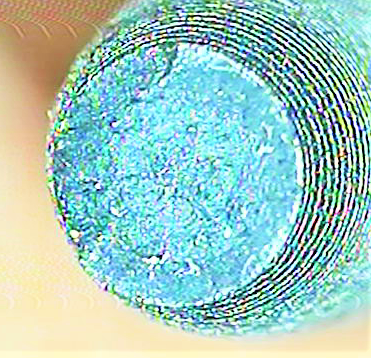
\includegraphics[width=6cm]{41.png}
		\caption{金相显微镜下低碳钢断口}
	\end{minipage}
	\begin{minipage}[t]{0.48\textwidth}
		\centering
		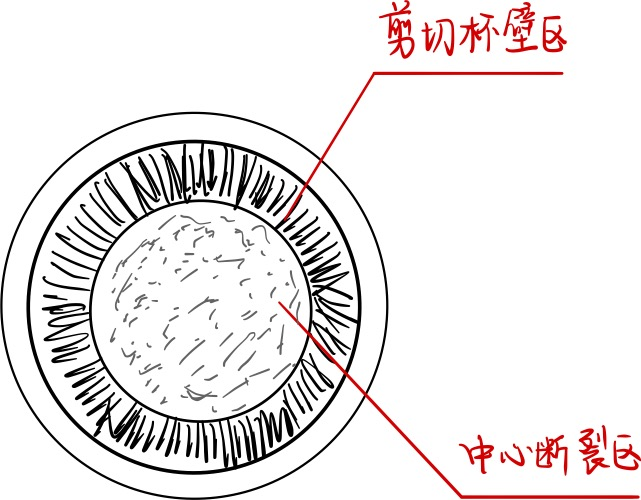
\includegraphics[width=6cm]{42.jpg}
		\caption{试件断口分区}
	\end{minipage}
\end{figure}
\begin{enumerate}
	\item[1] 中心断裂区:断裂面凹凸不平非常明显
	\item[2] 边缘断裂区:周边成$45\deg$倾斜,较为光滑平整,杯状断裂面
\end{enumerate}

\subsection{试件断口附近应力分析}
塑性材料在拉应力作用下会发生颈缩现象,这个现象导致杯壁剪切区(如图所示) 成三向应力状态,沿 $ 45\deg $ 角度发生剪切断裂。材料发生颈缩时,其内部由单向应力状态变成三向应力状态。在三向应力状态下,中心部分应力变大,发生脆性断裂。中心部分的晶粒被拉长,不再保持原来的状态,因此可以观察到断口的颜色发生改变。并且中心断裂区域的颜色与杯口区域的颜色不同中心部分的颜色较暗,断面非常粗糙;而两边的颜色稍亮,断面比较光滑。这是因为中心断裂区发生了脆性断裂,而中心断裂区脆性断裂发生后形成微孔,微孔沿$ 45\deg $ 方向向两边扩展,造成两边的剪切断裂,此处断面较光滑。如图所示
\begin{figure}[htbp]
	\centering
	\begin{minipage}[t]{0.48\textwidth}
		\centering
		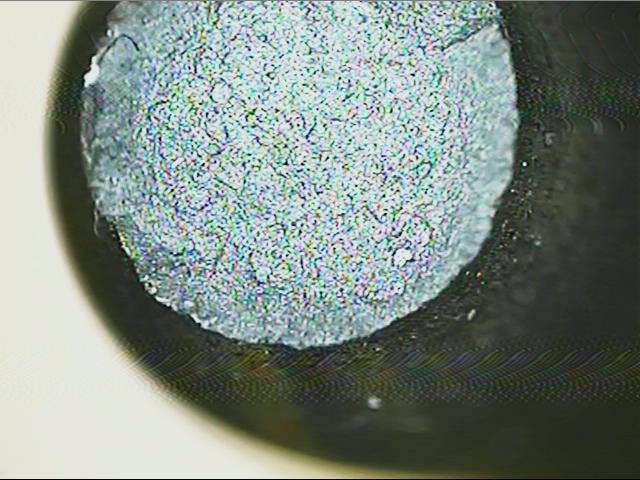
\includegraphics[width=6cm]{43.jpg}
		\caption{断面的显微照片}
	\end{minipage}
	\begin{minipage}[t]{0.48\textwidth}
		\centering
		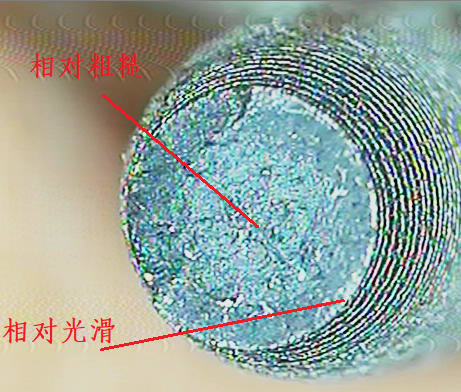
\includegraphics[width=6cm]{43.png}
		\caption{中心断裂区与边缘断裂区的对比}
	\end{minipage}
\end{figure}

由于广义胡克定律
\begin{equation}
	\epsilon_1 =\frac{1}{E} \left[\sigma_1 - \mu (\sigma_2 + \sigma_3)\right]
\end{equation}
$ \sigma_2 $ 和 $ \sigma_3 $ 不会过大,因此中心部分的切应力 $ \tau $ 也不会太大,从而中心部分不会发生剪切断裂,反而会发生脆性拉断。

\subsection{低碳钢的颈缩过程}

讨论完以低碳钢为例的塑性材料的断裂过程,需要讨论一下试件克服屈服极限后发生的颈缩过程。颈缩过程中的断面侧面图所示

\begin{figure}[htbp]
		\centering
		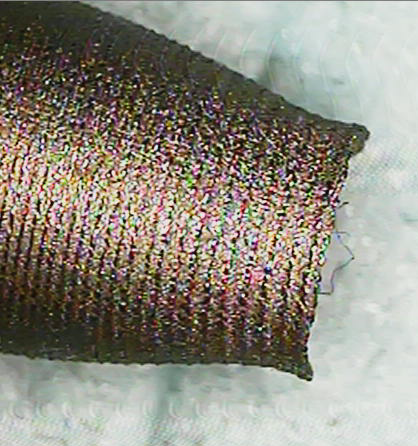
\includegraphics[width=10cm]{44.png}
		\caption{低碳钢断口侧面显微照片}
\end{figure}
从断口侧面图可以看出,在颈缩过程中,试件表面的晶格已经发生变化,晶格拉伸和破坏的方向与正应力的方向相同。由于颈缩时材料局部塑性变化,而且截面面积变小,材料内部的不均匀属性开始体现,可以看出试件表面出现环状圆周凸起,而且越靠近颈缩区越凸起越显著。

\section{灰铸铁的断面图}

\begin{figure}[htbp]
	\centering
	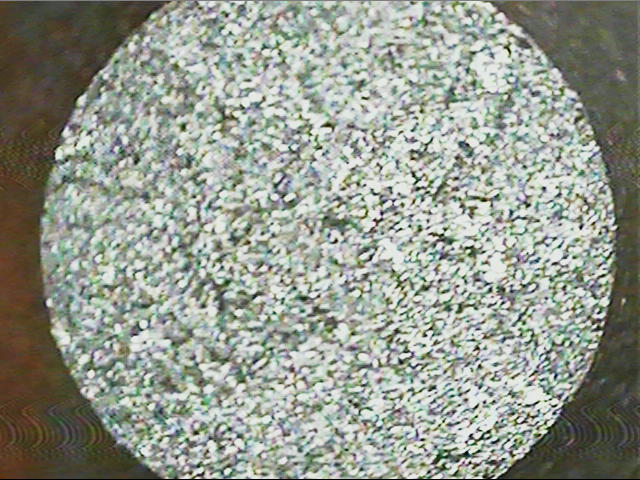
\includegraphics[width=10cm]{45.png}
	\caption{灰铸铁断面金相显微照片}
\end{figure}	

灰铸铁在拉伸中发生了脆性破坏,断面近似呈平面,断面有微小起伏,断面没有出现颈缩现象。说明灰铸铁的断裂是材料不能抵抗轴向拉应力而发生的脆性破坏。
\end{document}
